\subsubsection{State in the Repl}
As Haskell encapsulates state within monads, any function which seeks to manipulate state must be
within that monad. This was most important in the type inference module and in the repl, where new
function definitions had to be dynamically added to the environment and type-checked.
Figure~\ref{fig:exec}

\begin{figure}
    \begin{minted}[breaklines=true]{haskell}
        -- | execution function while repl is running
        exec :: Bool -> L.Text -> Repl ()
        exec update source = do
            st       <- get

            mod'     <- hoistError $ parseProgram "<stdin>" source
            typeEnv' <- hoistError $ inferTop (typeEnv st) mod'

            let st' = st { termEnv = foldl' evalDef (termEnv st) mod'
                         , typeEnv = typeEnv' `mappend` typeEnv st 
                         }

            when update (put st')

            case Prelude.lookup "it" mod' of
              Nothing -> return ()
              Just ex -> do
                let (val, _) = runEval (termEnv st') "it" ex
                showOutput val st'
    \end{minted}
    \caption{The exec function in Repl.Repl}
\label{fig:exec}
\end{figure}

\subsubsection{Type checking of built-in functions}
Primitive operators and functions, such as head and tail are not available to the inference engine.
Therefore it was necessary to `hard code' the type signatures into the environment, thereby allowing
students to check the type signature of various important functions, but also meaning that these
functions can now be type checked\footnote{Haskell overcomes this problem partially by having almost
everything as a library function, including such things as + and -, which in microML are
primitives.}. Figure~\ref{fig:typesigs}

\begin{figure}
    \begin{minted}[breaklines=true]{haskell}
          ("show"   , Forall  [polyA] (TVar polyA `TArrow` typeString))
        , ("read"   , Forall  [] (typeString `TArrow` typeNum))
        , ("ord"    , Forall  [] (typeChar `TArrow` typeNum))
        , ("chr"    , Forall  [] (typeNum `TArrow` typeChar))
    \end{minted}
    \caption{Hard-coded type signatures, in Data.Map form}
\label{fig:typesigs}
\end{figure}

\subsubsection{A Parsec Parser Combinator}
An example of a typical parsing function. Complex regular expressions have been replaced with small
regular expressions and other parser combinators. Figure~\ref{fig:parsec}

\begin{figure}
    \begin{minted}{haskell}
        lambda :: Parser Expr
        lambda = do
            reservedOp "\\"
            args <- many varName
            reservedOp "->"
            body <- expr
            return $ foldr Lam body args
    \end{minted}
    \caption{The parser for microML anonymous functions}
\label{fig:parsec}
\end{figure}

Truncating floating-point representation in the repl is done using string manipulation. The choice
of three consecutive 0s is largely arbitrary. See Figure~\ref{fig:trunc} and
Section~\ref{floatingPoint}.
\begin{figure}
    \begin{minted}[breaklines=true]{haskell}
        truncate' :: Double -> Double
        truncate' = read . dropZeros . show
            where dropZeros x = head (split x) ++ "." ++ getValid (head (tail (split x)))
                  split       = splitOn "."
                  getValid s 
                      | "e" `isInfixOf` s  = s
                      | hasform s = if length s == 1 then s else  show $ read [head s] + 1
                      | take 3 s   == "000" = "0"
                      | otherwise  = head s : getValid (tail s) 

        hasform :: String -> Bool
        hasform (_:ys) = all (== '9') ys 
    \end{minted}
    \caption{The truncation function for doubles in the repl}
\label{fig:trunc}
\end{figure}

\subsubsection{Unit Testing}
Unit testing was conducted with the HSpec package\footnote{\url{https://hspec.github.io/}}.
Figure~\ref{fig:unit}

\begin{figure}
    \begin{minted}[breaklines=true]{haskell}
        listprims :: IO ()
        listprims = hspec $ 
            describe "listprims" $ do
                describe "car" $ do
                    it "gets the head of a list" $ 
                        car (BinOp OpCons (Lit (LInt 3)) Nil) `shouldBe` (Lit (LInt 3) :: Expr)
                    it "gets the head of a string" $
                        car (Lit (LString "hello")) `shouldBe` (Lit (LChar 'h') :: Expr)
                    it "should fail on non-list ints" $ 
                        evaluate (car (Lit (LInt 1)))        `shouldThrow` anyException
                    it "should fail on non-list doubles" $ 
                        evaluate (car (Lit (LDouble 1)))     `shouldThrow` anyException
                    it "should fail on non-list chars" $ 
                        evaluate (car (Lit (LChar 'a')))     `shouldThrow` anyException
                    it "should fail on non-list bools" $ 
                        evaluate (car (Lit (LBoolean True))) `shouldThrow` anyException
    \end{minted}
    \caption{Unit testing}
\label{fig:unit}
\end{figure}


\section{Utilities}
MicroML also ships with a number of utility scripts.

The installation script is written in bash. Figure~\ref{fig:installation}
\begin{figure}
    \begin{minted}[breaklines=true]{bash}
        if [ -x "$stack" ]; then
            printf "\e[1mstack found\e[0m\n"
            printf "\e[1mrunning tests and building\e[0m\n"
            stack test 
            rc=$?
            if [[ "$rc" != 0 ]]; then
                printf "\n\e[31mCould not pass all tests. The build has failed\e[0m\n"
                exit "$rc" 
            fi
            printf "\e[1minstalling in $HOME/.local/bin/\n"
            stack install
            rc=$?
            if [[ "$rc" != 0 ]]; then
                printf "\nCould not install the executable into $HOME/.local/bin. Please copy it manually into your path\n"
                exit "$rc"
            fi
            printf "\n\e[1mcopying standard libraries to home directory\e[0m\n"
            ## delete old standard libs if they are found
            if [ -x "$HOME"/.microML ]; then
                printf "\n\e[1mremoving old standard library\e[0m\n"
                rm -rf "$HOME"/.microML
            fi
            printf "\n\e[1minstalling standard library\e[0m\n"
            cp -vr src/Libs "$HOME"
            mv "$HOME/Libs" "$HOME/.microML"
            printf "\n\e[1mcopying default .microMLrc to home directory\e[0m\n"
            cp -v utils/microMLrc "$HOME"/.microMLrc
            printf "\n\e[1mfinished!\e[0m\n"
        else 
            printf "\e[31mCould not find stack in your system path. Are you sure it's installed?\e[0]"
        fi
    \end{minted}
    \caption{Bash installation script}
\label{fig:installation}
\end{figure}

MicroML also has a simple (neo)vim plugin which ships with the repo. The folding function is of some
interest, as it autofolds comments, setting the function name as its `title'. See
Figures~\ref{fig:fold} and~\ref{fig:foldVim}

\begin{figure}
    \begin{minted}[breaklines=true]{vim}
        function! GetMMLFold(lnum) 
            let l:line = getline( a:lnum )

            " Beginning of comment
            if l:line =~? '\v^\s*--' || l:line =~? '\v^\s*(\*'
                return '2'
            endif

            if l:line =~? '\v^\s*$'
                let l:nextline = getline(a:lnum + 1)
                if l:nextline =~# '^--' || l:nextline =~? '^(\*'
                    return '0'
                else
                    return '-1'
                endif
            endif
            return '1'
        endfunction 
    \end{minted}
    \caption{Part of the folding function for vim}
\label{fig:fold}
\end{figure}

\begin{figure}
    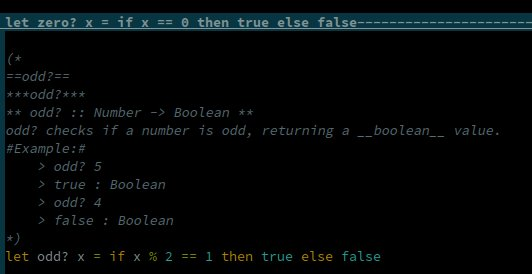
\includegraphics[width=\textwidth]{images/vim.jpg}
    {\caption{Folding and syntax highlighting in the editor}}
\label{fig:foldVim}
\end{figure}
